%%%%%%%%%%%%%%%%%%%%%%%%%%%%%%%%%%%%%%%%%%%%%%%%%%%%%%%%%%%%%%%%%%%%%%%%
% Preamble
%%%%%%%%%%%%%%%%%%%%%%%%%%%%%%%%%%%%%%%%%%%%%%%%%%%%%%%%%%%%%%%%%%%%%%%%
\documentclass[11pt]{article}
%
% Packages and other includes
% Pagination
\usepackage[letterpaper, margin=1.25in]{geometry}
%
% Graphics, floats, tables
\usepackage{graphicx, color, float, array}
%
% Hyperlinks
\usepackage{hyperref}
%
% AMS packages for equations, math symbols
\usepackage{amsmath, amssymb, braket}
%
% Bibliography
\usepackage[style=numeric,sorting=none]{biblatex}
\addbibresource{referencesProject2.bib}
%
% Revision (see Makefile)
\newcommand{\Revision}{977be36}

%
% Definitions and settings
% Paragraph indent and spacing
\setlength{\parskip}{0.4\baselineskip}
\setlength{\parindent}{0in}
%
% Math mode version of "r" column type (requires array package)
\newcolumntype{R}{>{$}r<{$}}
% comment format
\newcommand*{\comment}[1]{{\color{blue} #1}}
%
% Title, authors, date
\title{\textbf{3-Br versus 5-Br substitution on luciferin}}
\author{Brian Nguyen and Luke Nambi}
\date{Chem 150L Winter 2018 \\ \today, Revision \Revision}
%
%
%%%%%%%%%%%%%%%%%%%%%%%%%%%%%%%%%%%%%%%%%%%%%%%%%%%%%%%%%%%%%%%%%%%%%%%%
% Main document
%%%%%%%%%%%%%%%%%%%%%%%%%%%%%%%%%%%%%%%%%%%%%%%%%%%%%%%%%%%%%%%%%%%%%%%%
%
\begin{document}

\maketitle

\begin{abstract}
  \noindent
%  The abstract should contain a concise summary of the
%  question/hypothesis investigated (first sentence), state the methods
%  that were used to address it (second sentence), followed by a summary
%  of the most important results (1-2 sentences), and the main
%  conclusions (1-2 sentences). The abstract should be written in present
%  tense.
  The bromine substitution in the 5-bromoluciferin and 7-bromoluciferin are
  investigated to discover which halogen group substitution 
  may strengthen the
  fluorescent emission and red-shift the emission in 
  comparison to luciferin.
  The predicted excited states properties 
  and the computed einstein coefficient
  show that 5-bromoluciferin is a viable candidate for further development
  and characterization. The large einstein coefficient of 5-bromoluciferin
  correlates with the bioluminescent 
  intensity experiments and this indicates
  the efficient use of computations 
  to direct future development of bioluminescent
  biomarkers.
\end{abstract}

\section{Introduction}

Fluroscent labels are crucial to obtain spatial resolution of
chemical processes in a cell or in tissue - by labelling
proteins or enzyme substrates, various chemical processes
including chemical uptake and cellular transport can be
monitored. Good labels will have a high rate of spontaneous
emission (a high Einstein Coefficient) as well as emission at a
a red-shifted emission wavelength that is not absorbed by the
celluar matrix is hence ideal.\cite{doi:10.1002/cbic.201600564} Discovering
new fluroscent labels is a difficult
task without computation as there are no direct
means of predicting excited state properties and emission
from ground state lewis structures. It is expected that a
bromine substituion on the fused ring of luciferin
would red-shift the emission.

By computing the excitation and de-excitation properties of two
luciferin with a bromine subsitutient, an estimate of the rate of
spontaneous emission of each compound in the gas phase can be made.
The estimate can be used to guess at which bromo-substituted
luciferin compound would be a better fluoresent label in the
presence of luciferase in a cell. In this study, the 5-bromoluciferin
(5-BrLuc) and the 7-bromoluciferin (7-BrLuc) are investigated
to determine if they are viable candidates for further characterization
and development of the next generation of bioluminescent markers. 

\section{Methods}

\subsection{Statement of the Models}

Excitation and de-excitation by the absorption and emission of a
single photon are linear spectroscopic phenomenon, well
described by linear response in Time Dependent Density
Functional Theory.  

Linear Response in Time Dependent Density Functional Theory is
often written as a psuedo-eigenvalue problem due to Casida,

\begin{equation}
   \label{eq:Casida}
   \left(\begin{array}{cc}\mathbf{A}-\mathbf{\Omega}&\mathbf{B}\
     \\\mathbf{B}&\mathbf{A}+\mathbf{\Omega}\end{array}\right)\
   \left(\begin{array}{cc}\mathbf{X}\\\mathbf{Y}\end{array}\right)\
   =\
   \left(\begin{array}{cc}\mathbf{P}\\\mathbf{Q}\end{array}\right).
\end{equation}

A comprehensive description of each term is not included here
in interest of length. $ \mathbf{\Omega} $ is a vector containing all the
excitation energies of the system. Solving for the first few
indices of $ \mathbf{\Omega}$ gives the first few excitation energies of
system (i.e. $ \omega_{12}$,$\omega_{13}$,$\omega_{14}$ etc.)
while other properties can be obtained from the corresponding
$(\mathbf{X+Y})$ and $(\mathbf{X-Y})$. 
For example, the lowest energy excitation
has the excitation energy $ \omega_{12} $ and eigenvectors
$(\mathbf{X+Y})_{12}$ and $(\mathbf{X-Y})_{12}$ .

An adaptation of this linear response is presented by Furche,
using a density matrix based approach, resulting in a
relatively straight-forward calculation for the complete
difference density matrix for a single
excitation.\cite{doi:10.1063/1.1508368}

The traditional Z vector equation, 
$ \mathbf{Z}$ for a particular excitation is 
\begin{equation}
   \label{eq:Zvector}
   (\mathbf{A}+\mathbf{B})\mathbf{Z} = -\mathbf{R}
\end{equation}

describing the differences in the $ occ \times virt $ portion of
the difference density matrix. $\mathbf{R}$ contains both parts
of the excitation vector. An unrelaxed difference density matrix
$\mathbf{T}$ is defined, described the difference density matrix
for the  $occ \times occ$  and $virt \times virt$ parts of
the difference density matrix.

\begin{align}
  \label{eq:tEquation}
  \mathbf{T}_{occ\times occ} &= -\frac{1}{2}(\
  \mathbf{(X+Y)}_{occ\times vert}\mathbf{(X+Y)}^T_{occ\times vert}\ 
 +\mathbf{(X-Y)}_{occ\times vert}\mathbf{(X-Y)}^T_{occ\times vert}\ 
  )\\
  \mathbf{T}_{virt\times virt} &= \frac{1}{2}(\
  \mathbf{(X+Y)}^T_{occ\times vert}\mathbf{(X+Y)}_{occ\times vert}\ 
 +\mathbf{(X-Y)}^T_{occ\times vert}\mathbf{(X-Y)}_{occ\times vert}\ 
  )
\end{align}

The total difference density matrix can hence be thought of as
summing all the above, to cover the full dimensions of all
occupied and virtual molecular orbitals.

\begin{equation}
   \label{eq:pEquation}
   \mathbf{P} = \mathbf{T}_{occ \times occ} +\
                \mathbf{Z}_{occ \times virt} +\
                \mathbf{Z}^T_{occ \times virt} +\
                \mathbf{T}_{virt \times virt}
\end{equation}

The oscillator strength $|f|$, the change in the electronic dipole
moment during the electronic transition is therefore an
expectation value, where $\hat{\mathbf{\mu}}$ is the electric dipole
operator in 3 dimensions. 

\begin{equation}
\label{eq:oscilStrength}
|f|=|tr((\mathbf{P})\hat{\mathbf{\mu}})|
\end{equation}

Similarly, the energy gradient with respect to changing nuclei
position is also a trace of the total difference density matrix
with the nuclei displacement operator.

In summary, given reference state KS-orbitals, it is thus straight-forward
to solve for these excitation vectors with their
excitation energies.  From these excitation vectors, it
is possible to find the energy gradient with respect to
changes in nuclei positions and optimize the geometry
in an excited state. Also from the excitation vectors, it is then
possible to calculate the excitation transition dipole moment
or the oscillator strength, and from there the einstein
coefficient $A$ can be calculated. $ c $ is the speed of light,

\begin{equation}
  \label{eq:EinsteinCoeff}
  A_{21} = \frac {2(\omega_{21})^2 |f_{21}|} {c^3}
\end{equation}

where $|\omega_{21}|= |\omega_{12}| $ 
and $|f_{21}|= |f_{12}| $. The calculations were all
in atomic units, with a final conversion to S.I. units
at the end. Most constants are equal to 1, in atomic units
and are omitted in the equations above. The calculation is
approximate due to finite basis sets, the lack of an exact
exchange-correlation kernal, and other numerical
approximations in integrals.

\subsection{Computational Details}

Calculations were performed with {\sc Turbomole}
7.2.1\cite{TURBOMOLE}. Geometry optimization with
the closed-shell ground state electronic structure
was first conducted in the gas phase with DFT.
Based on this ground state geometry and electronic structure, a
linear response TDDFT calculation with full response is carried
out. Subsequently, a geometry optimization with the first excited
singlet state is carried out with the same full response TDDFT.
As a result, the excitation energies and oscillator strengths
are already computed. Based on the benchmarks, the best
functional for these sorts of calculations is the PBE0 hybrid
functional\cite{doi:10.1063/1.478522}. Given that the hydrogen
atoms do not participate significantly in the $\pi$to$\pi^*$ excitations,
it is reasonable to speed up the calculation with a basis set
with more functions on the important atoms. The def2-SV(P) basis
set was chosen\cite{Weigend.F:PCCP.2005}. The default threshold of
1E-7 for electronic structure convergence (\$scfconv) and 1E-3
for geometry convergence (-gcart) were used, with a gridsize
of m5 for numerical integration.\cite{Treutler95a}
Most of the information needed can be read directly from the
output file. Molden 4.6 was used to visual orbitals for
assigning transitions.

\section{Results $\&$ Discussion}

The vibrational spectrum for the optimized structures
at the ground and first excited states of 5-BrLuc and 7-BrLuc
is presented. The 5-BrLuc and 7-BrLuc optimized structures
are hence confirmed to be at a minimum with no imaginary frequencies.

\begin{figure}[H]
  \centering
  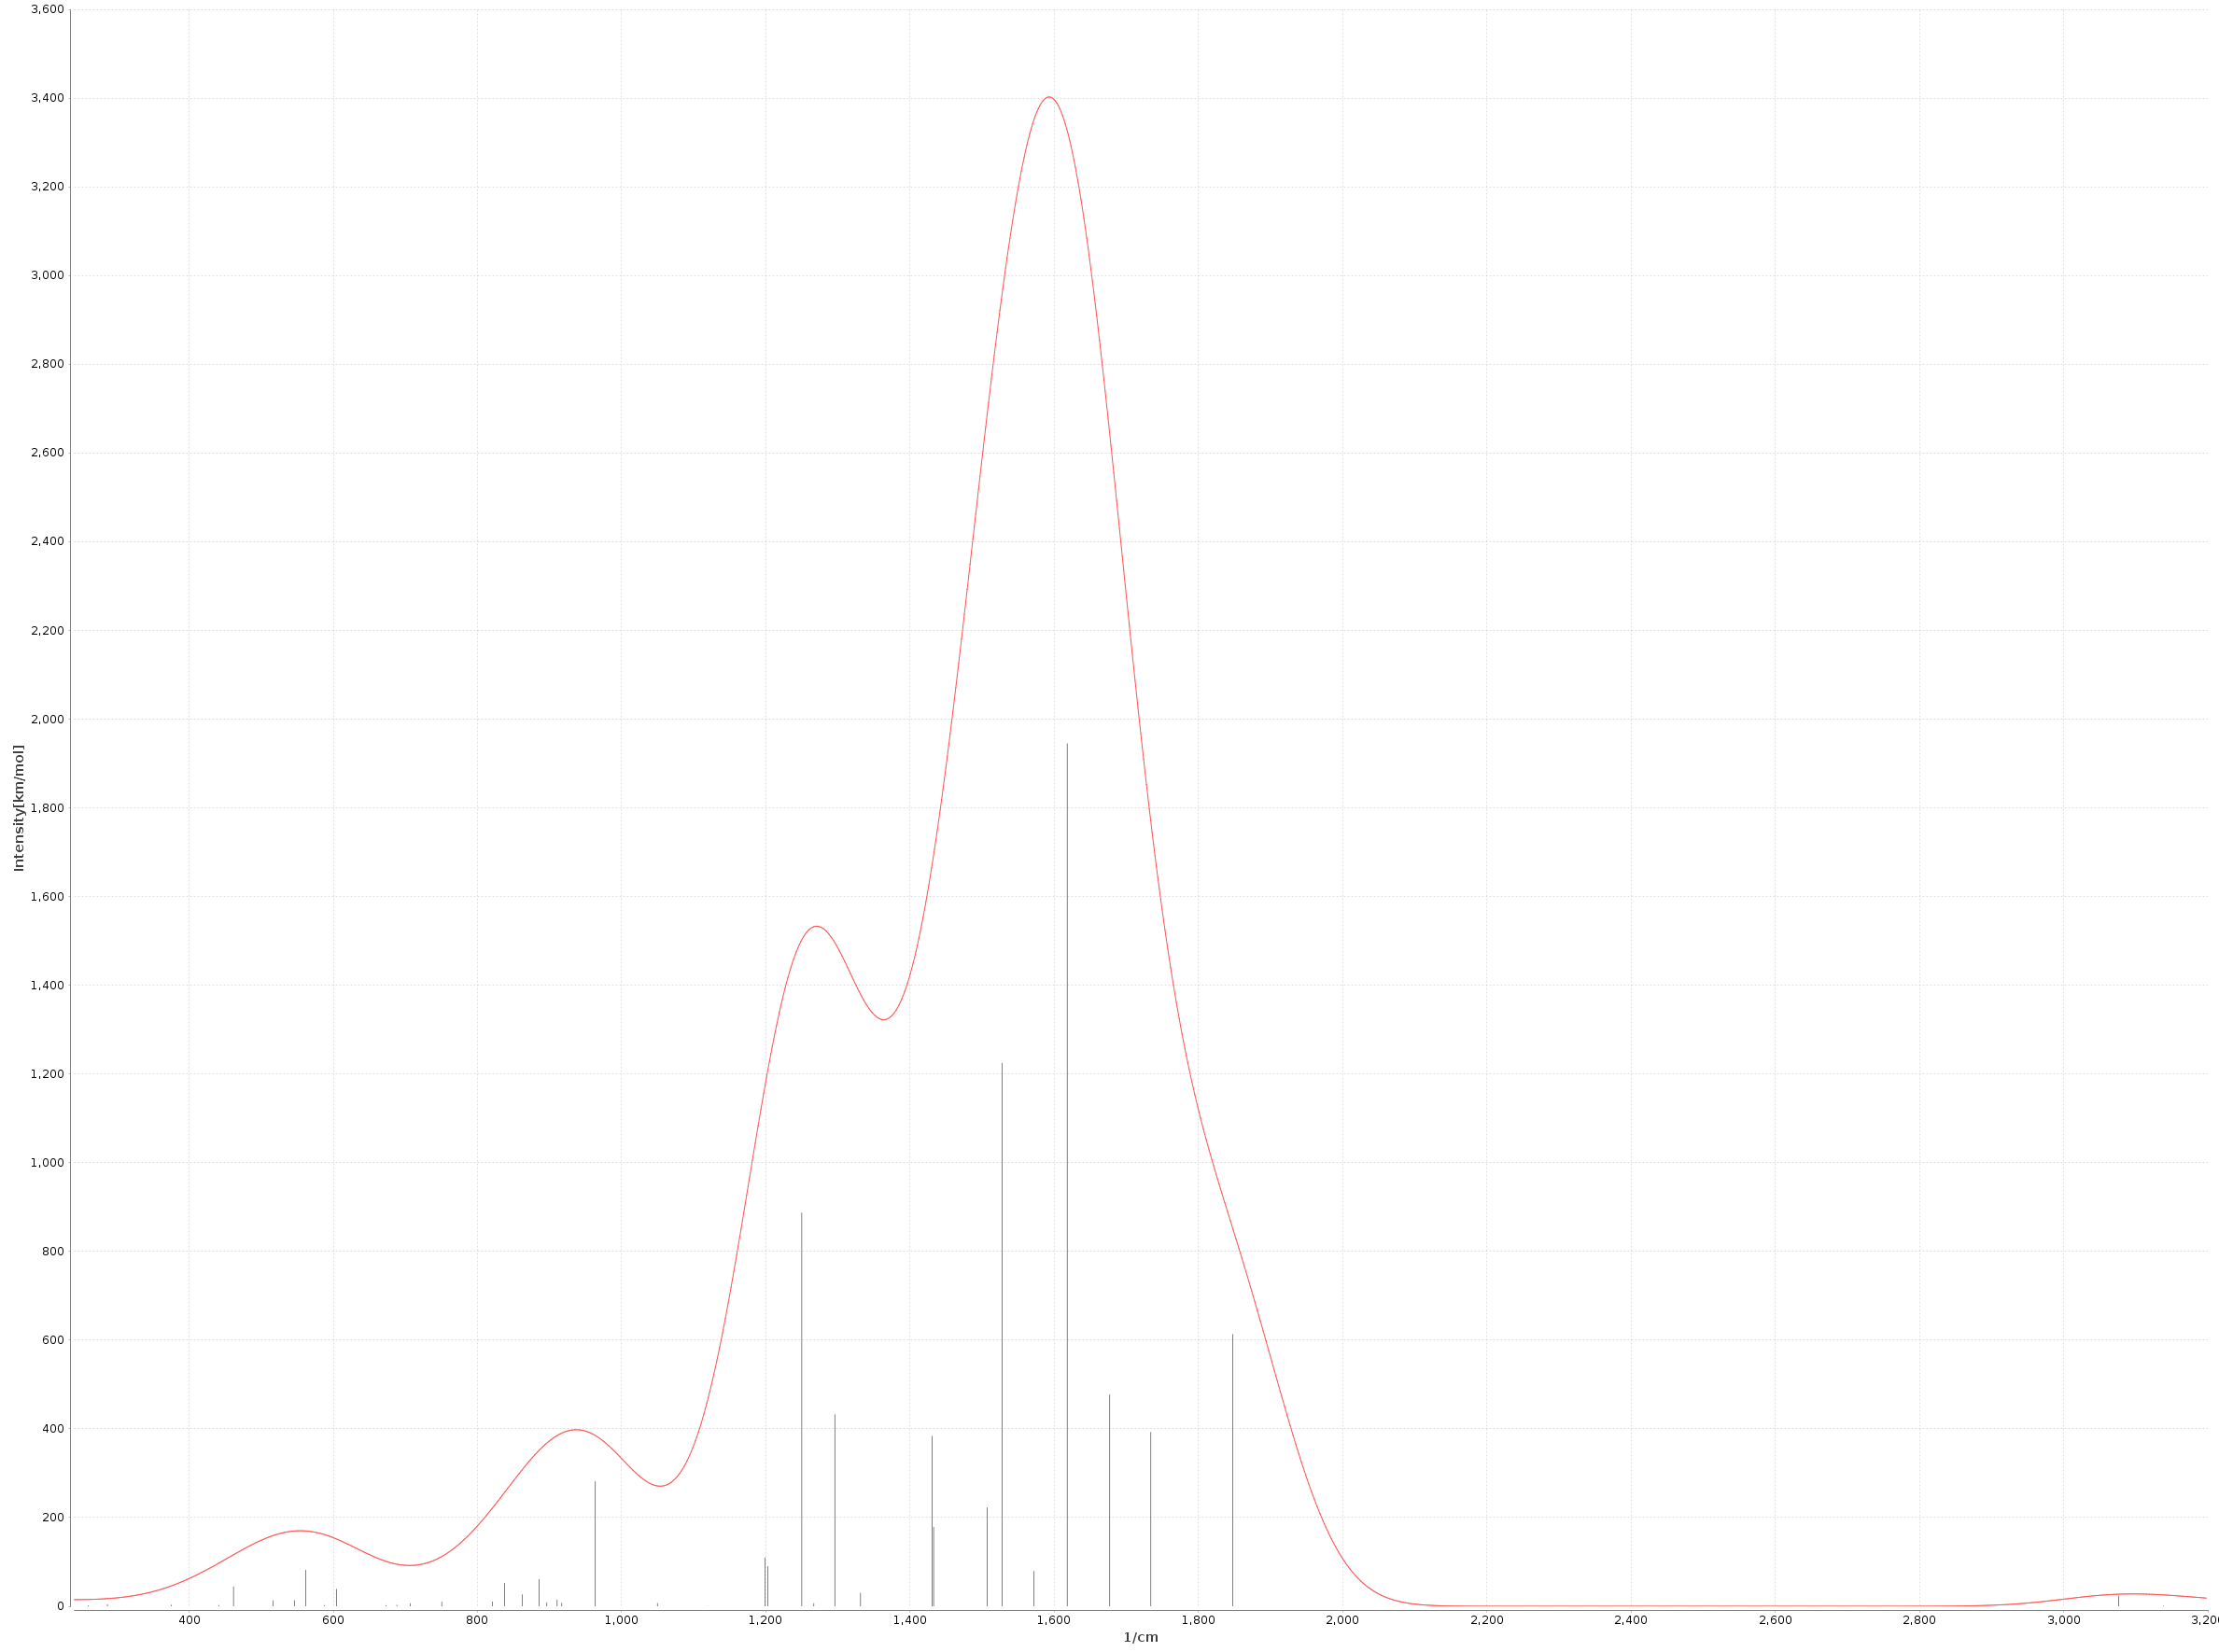
\includegraphics[scale=0.13]{ir_gs_5_brluc.png}
  \caption{Infrared spectrum of the optimized ground state 5-BrLuc
    using PBE0 functional with def2-SV(P) basis set.}
\end{figure}

\begin{figure}[H]
  \centering
  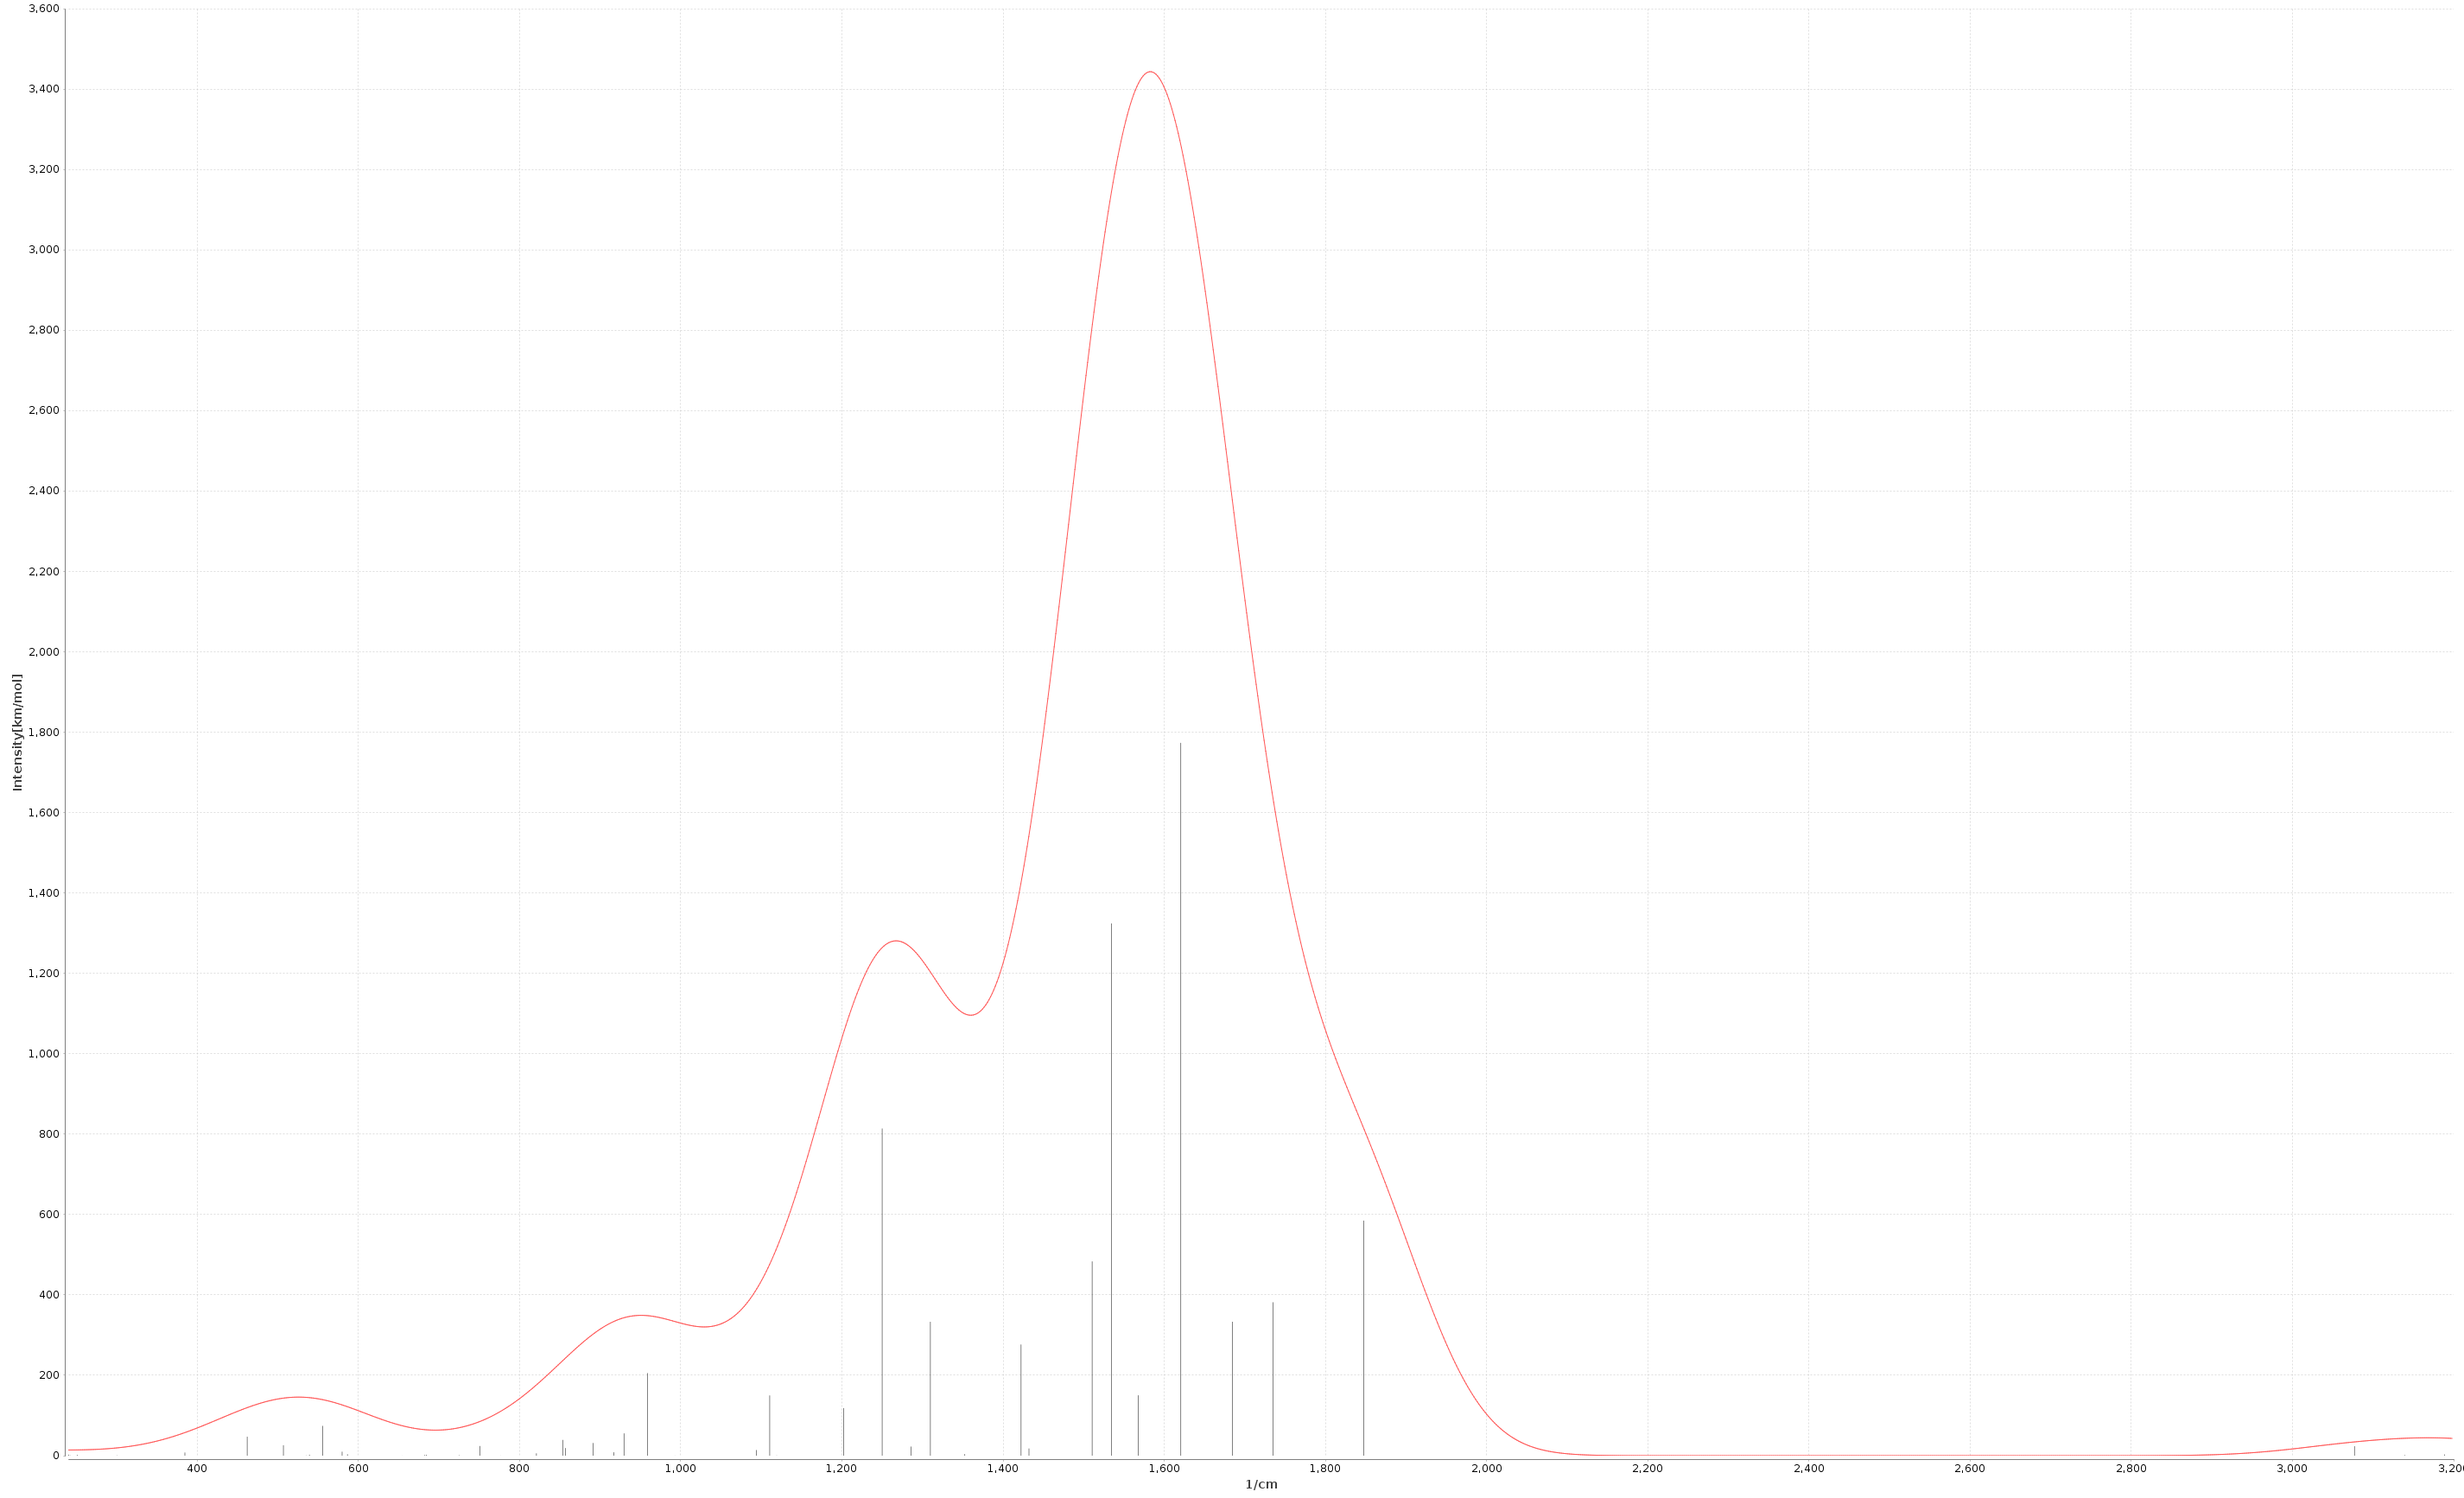
\includegraphics[scale=0.13]{ir_gs_7_brluc.png}
  \caption{Infrared spectrum of the optimized ground state 7-BrLuc
    using PBE0 functional with def2-SV(P) basis set.}
\end{figure}

\begin{figure}[H]
  \centering
  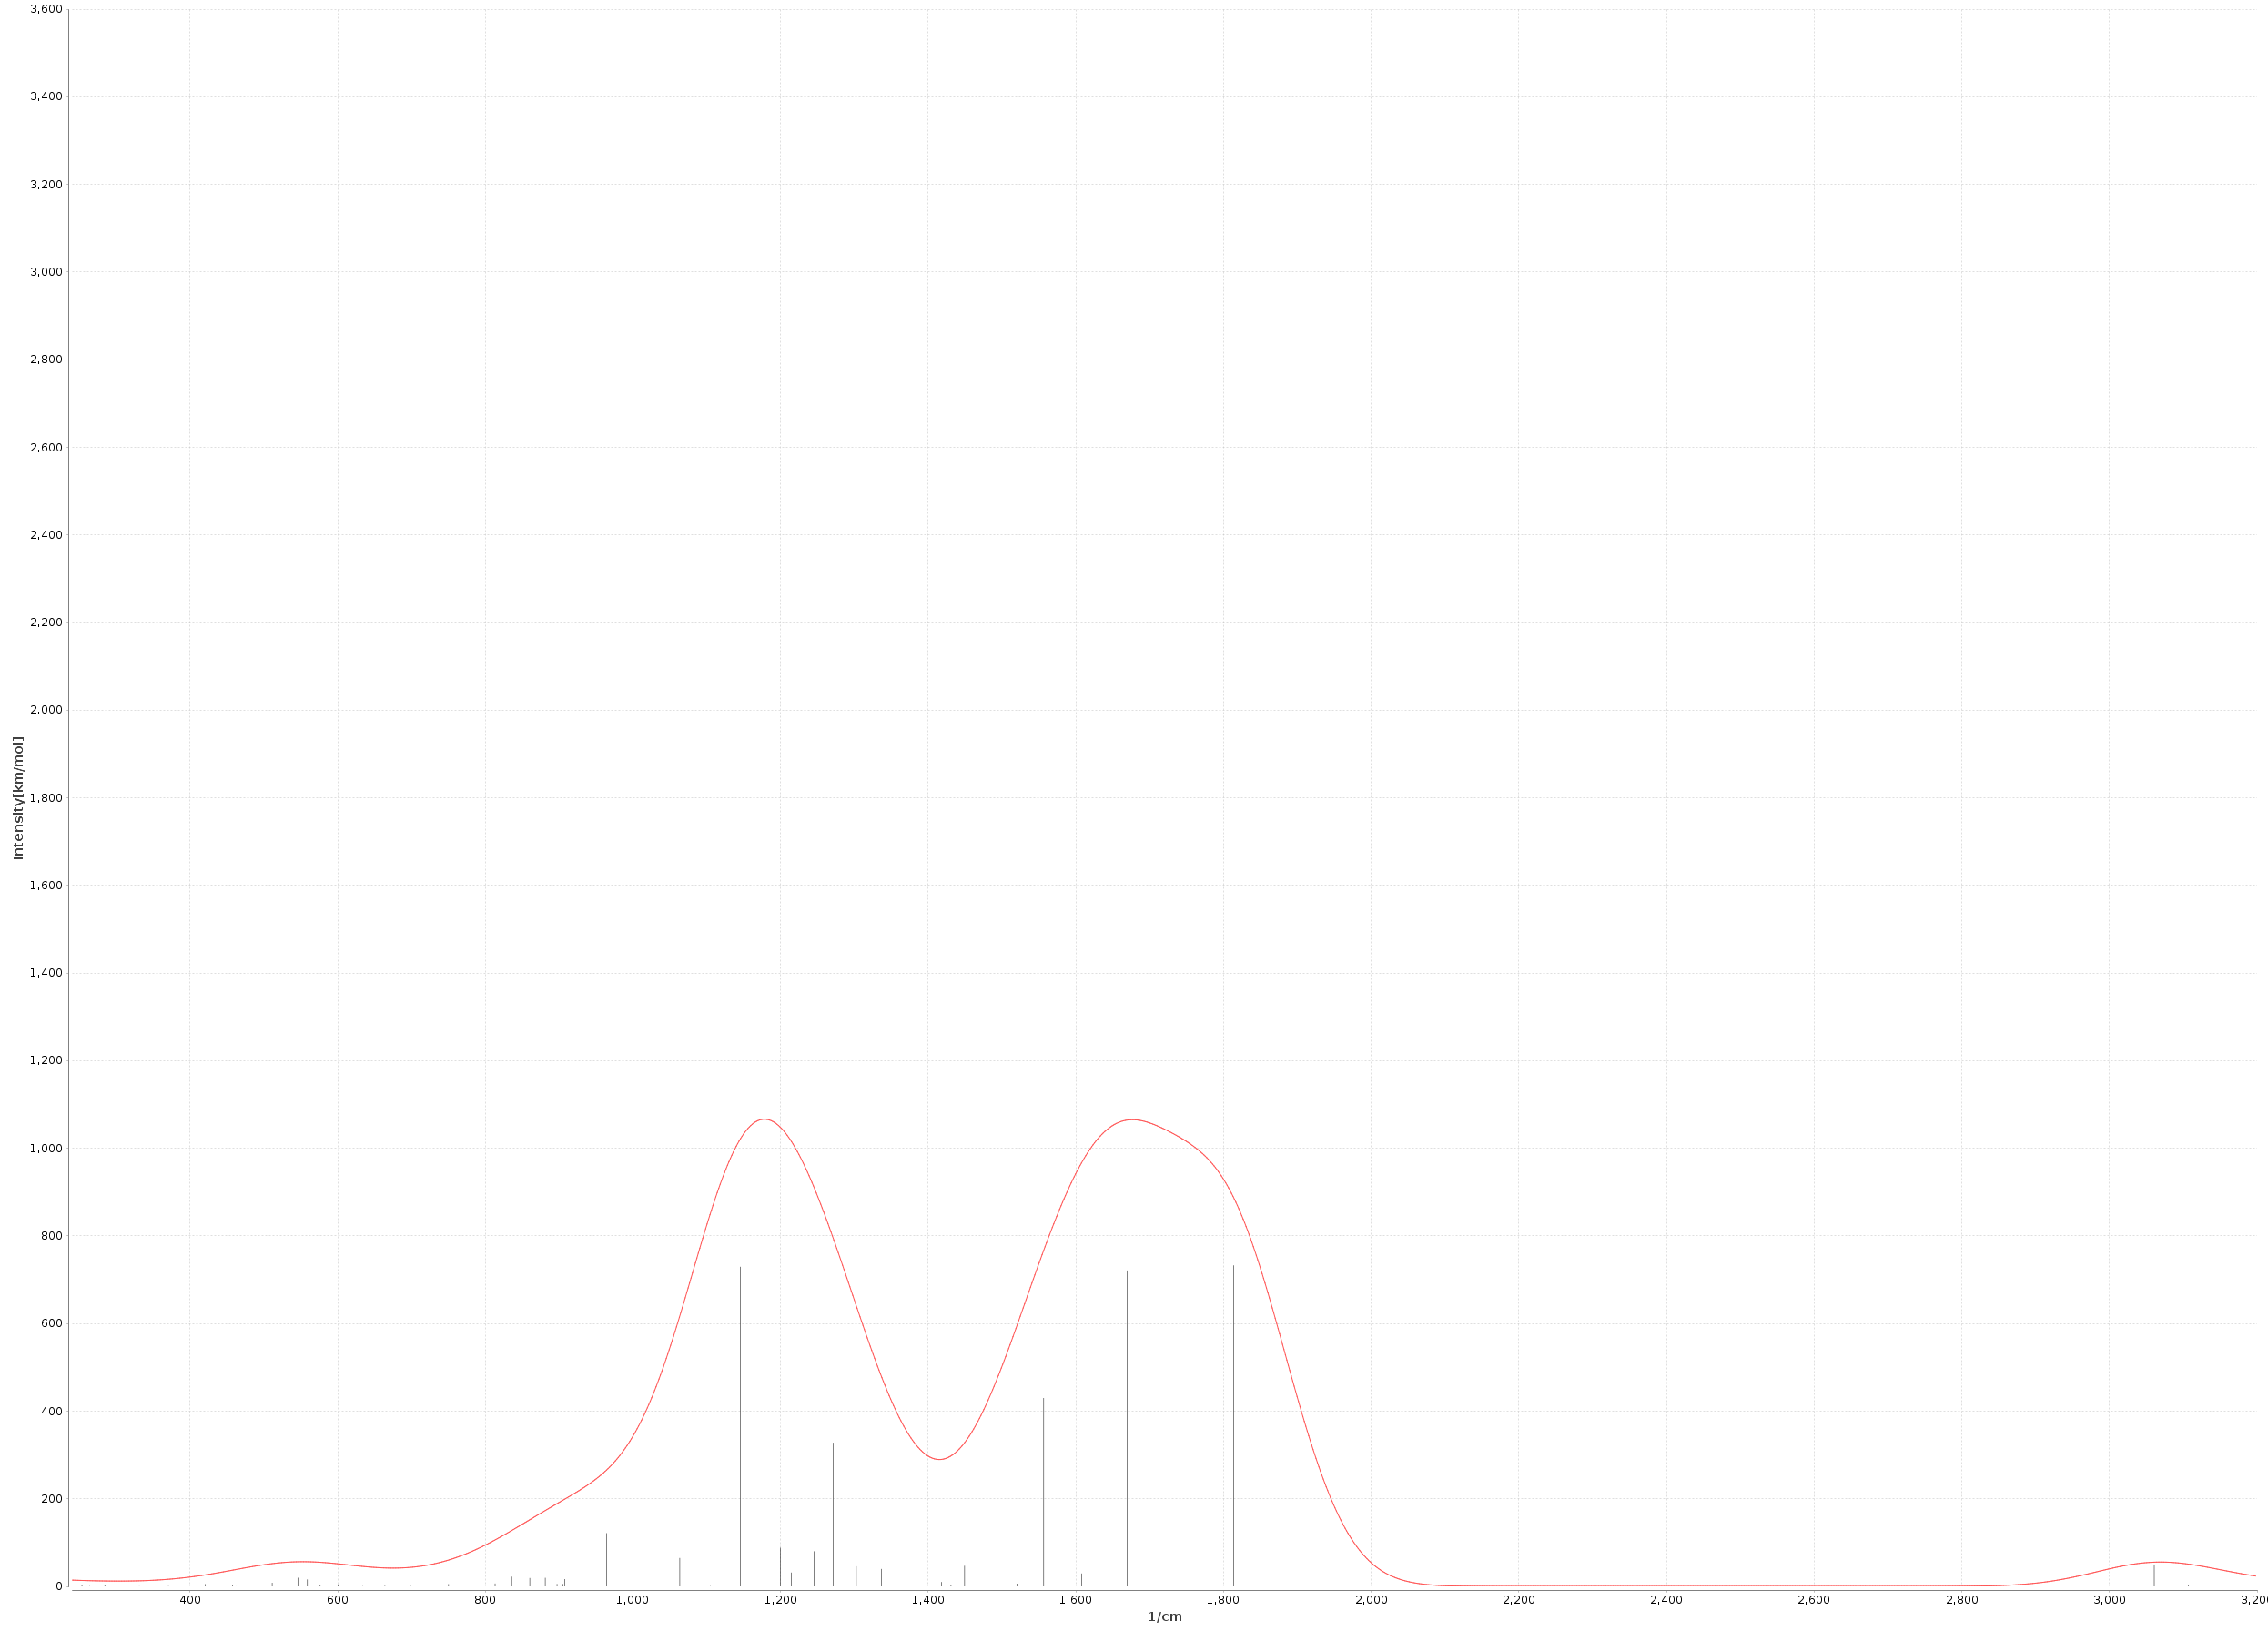
\includegraphics[scale=0.13]{ir_ex1_5_brluc.png}
  \caption{Infrared spectrum of the optimized first excited
    state 5-BrLuc using PBE0 functional with def2-SV(P) basis set.}
\end{figure}

\begin{figure}[H]
  \centering
  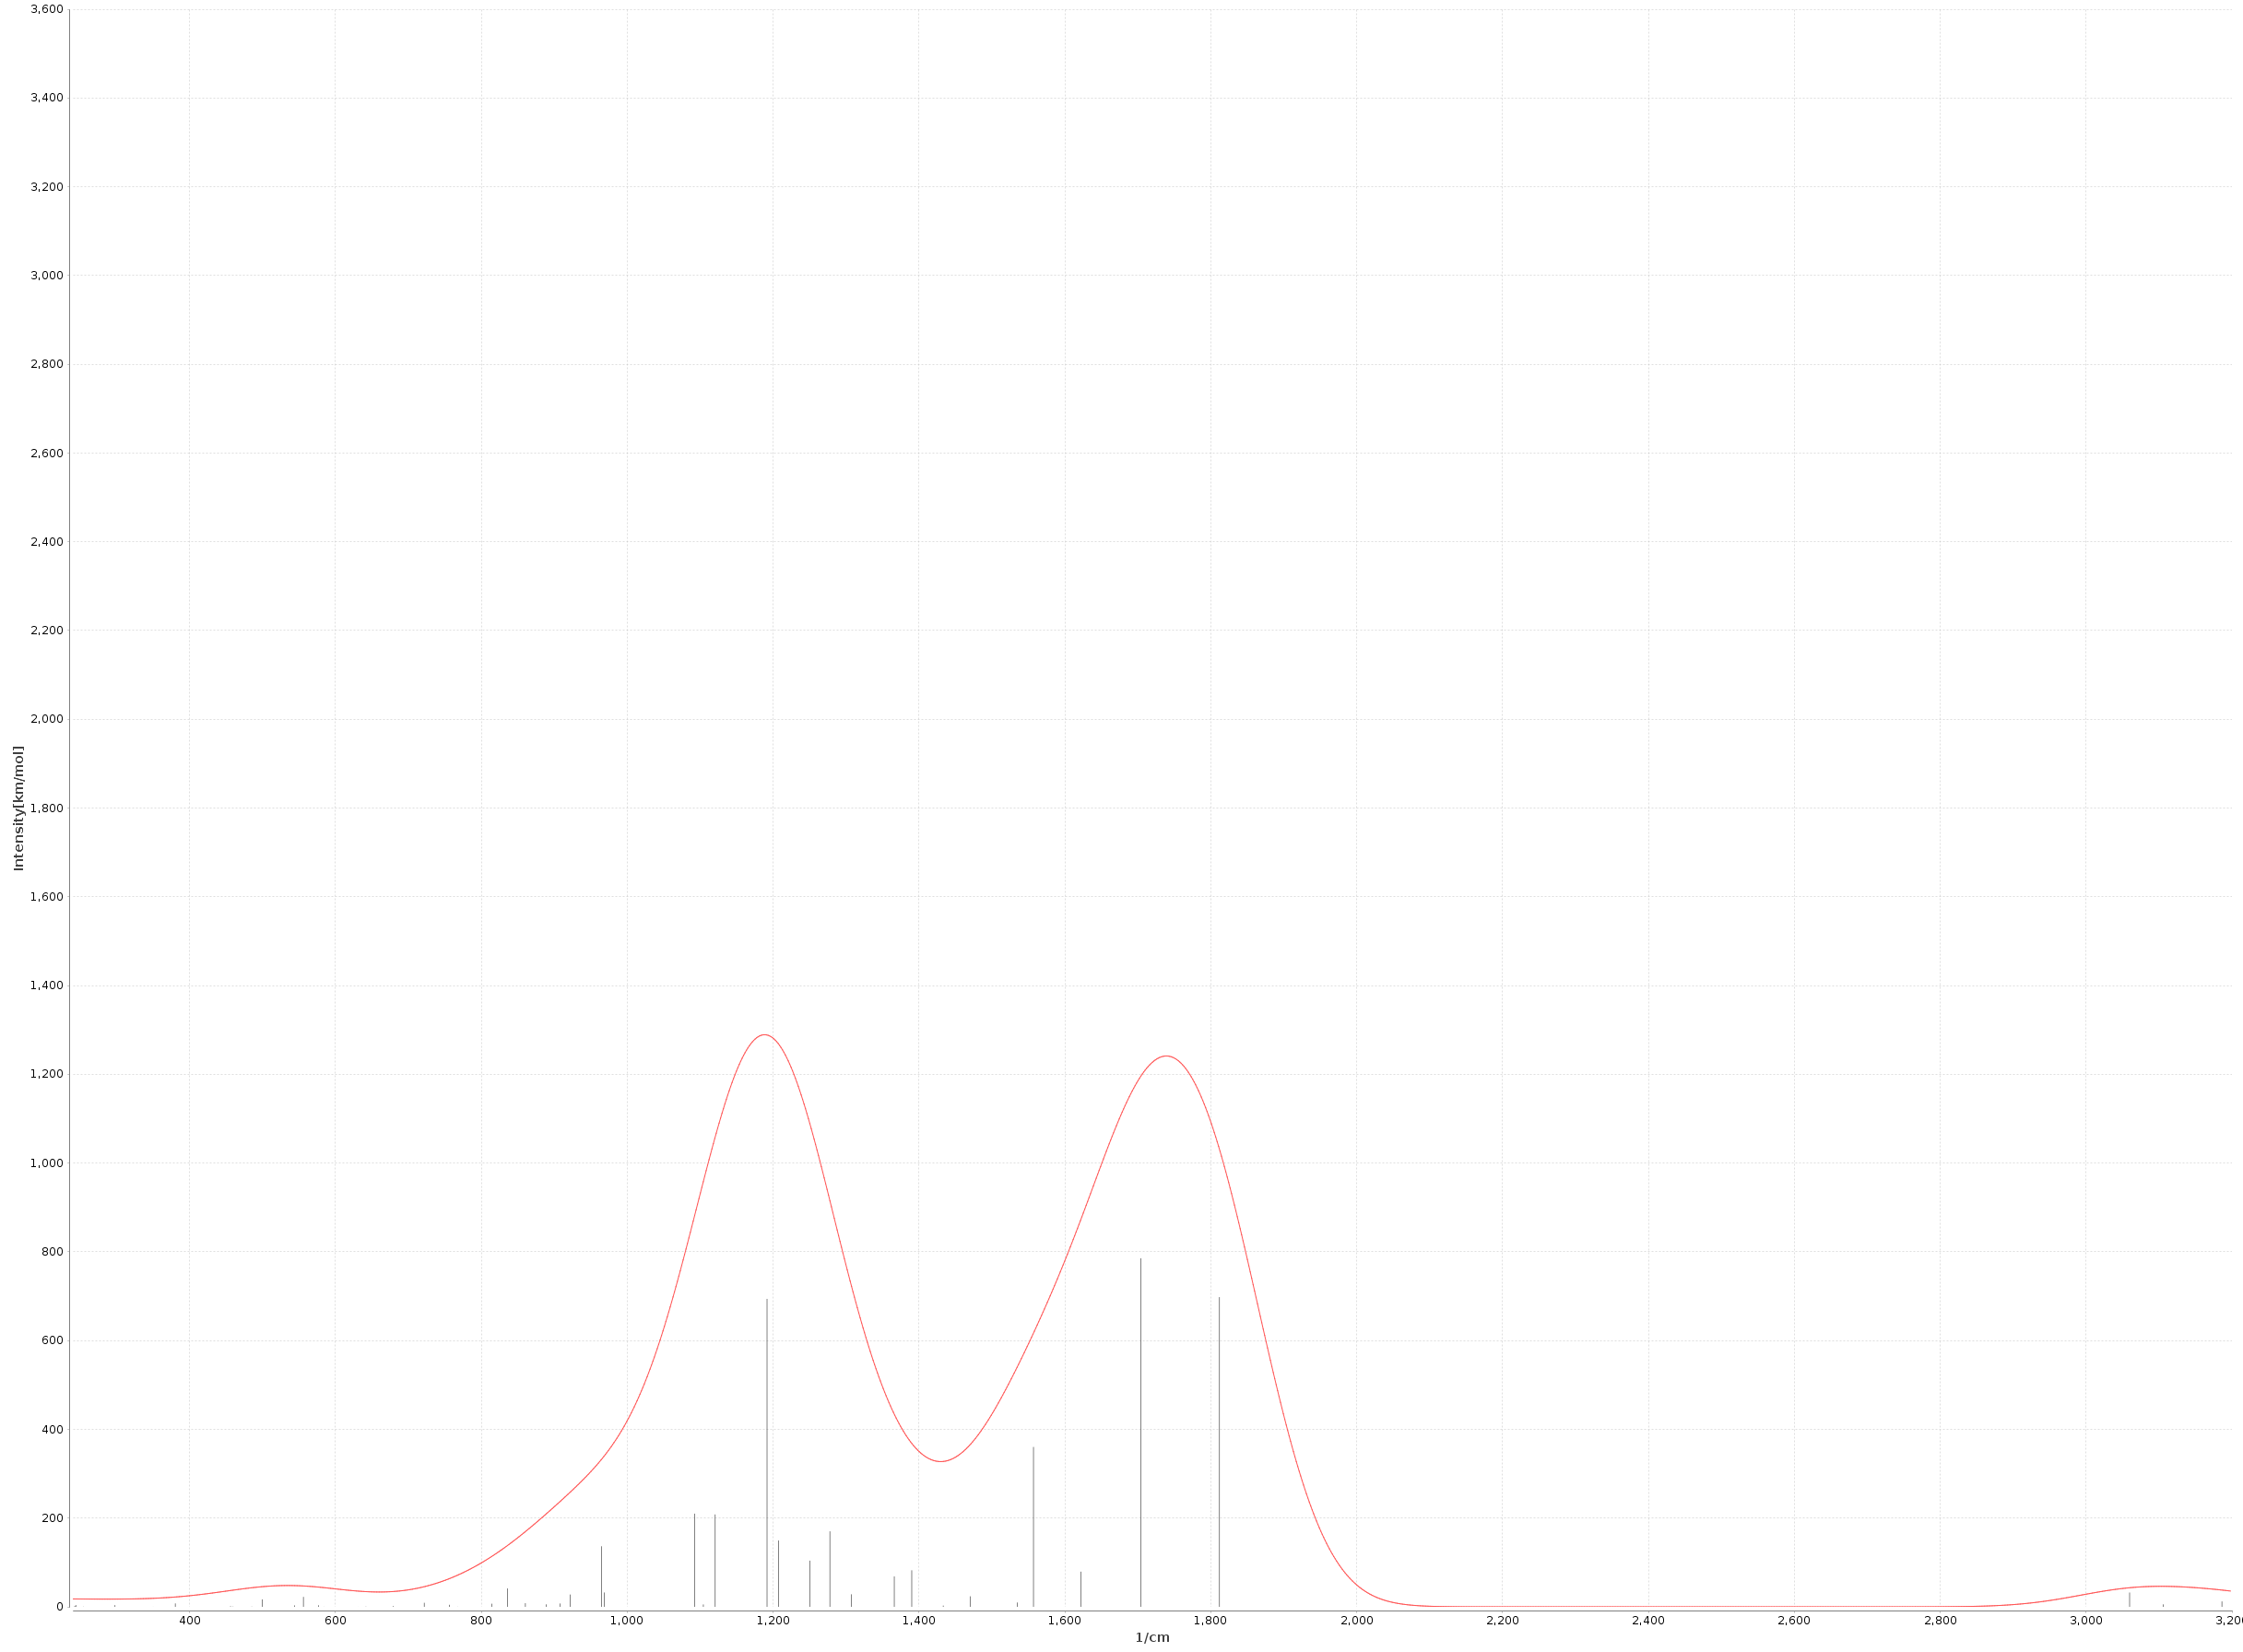
\includegraphics[scale=0.13]{ir_ex1_7_brluc.png}
  \caption{Infrared spectrum of the optimized first excited
    state 7-BrLuc using PBE0 functional with def2-SV(P) basis set.}
\end{figure}

\begin{table}[H]
 \centering
\begin{tabular}{|c|Rcc|}
  \hline
  Absorbances & \multicolumn{3}{c|}{5-BrLuc}  \\
  &Energy (nm)& Contribution & \\
  \hline
  1 &465.5826& HOMO $\rightarrow$ LUMO &0.940 \\
   & & $\pi$ $\rightarrow$ $\pi*$& \\
  \hline
  2 &407.0486& HOMO-1 $\rightarrow$ LUMO &0.967\\
   & & $nb_{O}$ $\rightarrow$ $\pi*$& \\
  \hline
  3 &356.2384& HOMO-2 $\rightarrow$ LUMO& 0.950 \\
   & & $\pi$ $\rightarrow$ $\pi*$& \\
  \hline
  \hline
  Absorbances & \multicolumn{3}{c|}{7-BrLuc}  \\
  &Energy (nm)& Contribution& \\
  \hline
  1 &474.9284& HOMO $\rightarrow$ LUMO & 0.933 \\
   &  & $\pi$ $\rightarrow$ $\pi*$ &\\
  \hline
  2 &405.7144& HOMO-1 $\rightarrow$ LUMO & 0.966 \\
   &  & $nb_{O}$ $\rightarrow$ $\pi*$ &\\
  \hline
  3 &342.4742 & HOMO-2 $\rightarrow$ LUMO & 0.934 \\
   & & $\pi$ $\rightarrow$ $\pi*$ &\\
  \hline
\end{tabular}
\caption{The reported wavelengths of the first three
  singlet excitations from the ground state geometry of
  5-BrLuc and 7-BrLuc.}
\label{tab:absorbance}
\end{table}

\begin{table}[H]
 \centering
\begin{tabular}{|c|Rcc|}
  \hline
  Fluoresence & \multicolumn{3}{c|}{5-BrLuc}  \\
  &Energy (nm)& Contribution & \\
  \hline
  1 &519.7586& HOMO $\leftarrow$ LUMO &0.921 \\
   & & $\pi$ $\leftarrow$ $\pi*$& \\
  \hline
  \hline
  Fluoresence & \multicolumn{3}{c|}{7-BrLuc}  \\
  &Energy (nm)& Contribution& \\
  \hline
  1 &546.8339& HOMO $\leftarrow$ LUMO & 0.917 \\
   & & $\pi$ $\leftarrow$ $\pi*$ &\\
  \hline
\end{tabular}
\caption{The de-excitation wavelengths reported from the
  first excited state geometry of the 5-BrLuc and 7-BrLuc.}
  \label{tab:fluorescence}
\end{table}

In Table \ref{tab:absorbance}, the reported excitation energy
of 7-BrLuc is lower than 5-BrLuc. Meanwhile,
the vertical de-excitations from the first excited state geometry
is given in the Table \ref{tab:fluorescence}. The experimental
fluorescence of 5-BrLuc and
7-BrLuc\cite{doi:10.1002/cbic.201600564} is approximately off by
10 nm compared to the computed values.

\begin{figure}[H]
  \centering
  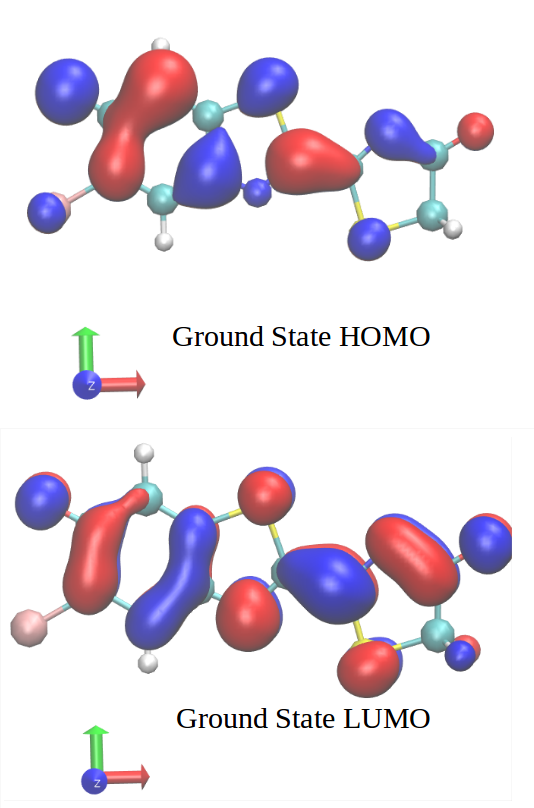
\includegraphics[scale=0.2]{compare_mos_5BrLuc.png}
  \caption{This is a comparison of the HOMO and LUMO of the
    5-BrLuc ground state structure, used to identify the
    excitation.}
  \label{fig:comp_5brLuc}
\end{figure}

\begin{figure}[H]
  \centering
  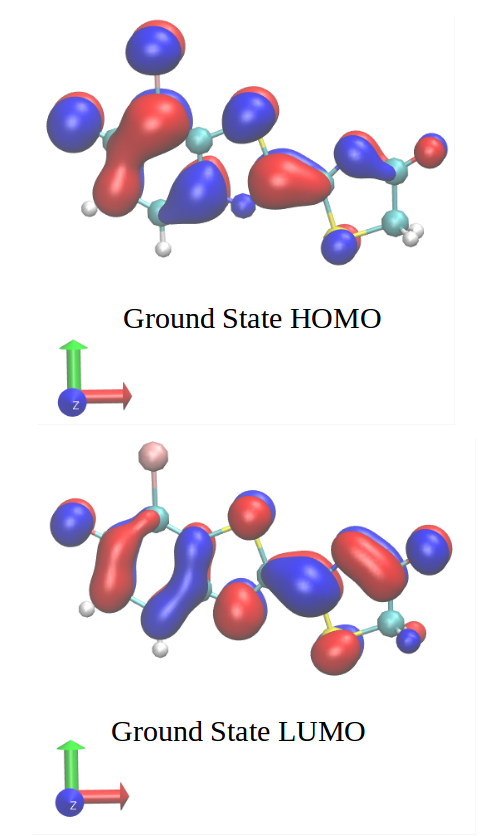
\includegraphics[scale=0.2]{7brluc_ex_gs.png}
  \caption{This is a comparison of the HOMO and LUMO of the
    7-BrLuc ground state structure, used to identify the
    excitation.}
  \label{fig:comp_7brLuc}
\end{figure}

With the oscillator strengths for fluoresence, the computed
einstein coefficients are: 5-BrLuc, $1.07e8$ photons per second,
and 7-BrLuc, $6.90e7$ photons per second. Relatively, the 5-BrLuc
einstein coefficient reveals that it is a strong emitter in comparison
to 7-BrLuc. This agrees with the bioluminescence
experiments\cite{doi:10.1002/cbic.201600564} from
a qualitative perspective.

\section{Conclusions}

%This section should aim to answer the hypothesis or question stated in
%the introduction clearly and concisely, as well as other possibly
%significant results of the study. Do not provide a summary of your work
%here, the correct place for that is the abstract. Instead, the
%conclusions must explain what has been learned, and how it is relevant to the
%initial question.

In summary, the 5-BrLuc is better candidate for the development of
the next generation of bioluminescent markers. The higher einstein
coefficient by approximately 10 fold make 5-BrLuc a stronger
emitter, even though the emission is slightly blue-shifted in comparison
to 7-BrLuc. The agreement with experimental work is encouraging
and suggests that computations can guide the experimental
work.

%\section*{Acknowledgments}
%
%This section should acknowledge any additional sources of support from
%professionals who aren't co-authors but helped you complete your work. For
%example, O. H. would like to acknowledge useful discussions with The
%Three Stooges. Often, funding agencies mandate that funding be
%acknowledged in this section. 

\printbibliography

\end{document}
